\documentclass[final, 3p,12pt,times,letter,twocolumn]{elsarticle}
\usepackage{graphicx}
\usepackage{booktabs}
\usepackage{multirow}
\usepackage{tabularx}
\usepackage[singlelinecheck = false]{caption}
\usepackage{array}
\usepackage{graphicx}
\usepackage{amsfonts}
\usepackage{amssymb}
\usepackage{natbib}
\usepackage{hyphenat}
\sloppy

\begin{document}

\journal{MScA, the University of Chicago}

\begin{frontmatter}
\title{Understanding and Predicting Online Customer Intention Based on their Browsing Behavior
\tnoteref{label1}}

\tnotetext[label1]{This paper is based on the course project of Data Mining Principles.}

\author{Qurat Ul Ain, Tamer Abousoud, Marcus Himelhoch, Jonathan Huff, Skye  Zhang}
\address{Graham School of Continuing Liberal and Professional Studies, the University of Chicago}
\begin{abstract}
In this study...... 
\\
\\
\\
\\
\\
\\
\\
\\

\end{abstract}

\begin{keyword}
Data Mining \sep Online Shopping\sep Customer intention\sep Browsing Behavior \sep Predictive Analytics \sep Recommendation System
\end{keyword}

\end{frontmatter}


\section{Introduction}
Since the invention at the end of the 19th century, online shopping has gradually become a major disruption of the retailing industry. To date, most of the companies have created beautifully designed and well organized websites to attract consumer to shop online. According to Sakar et al. (2018), online shopping in the past few years has created potential in the retailing market, but the fact is that the development on visual design hasn't triggered much conversion rate towards making an online purchase.

Van der Heijden et al. (2003) conceptualized the distinction between traditional retailing and online retailing in terms of the customer behavior. In general, online consumers behave differently from the traditional ones for two reasons: 
\begin{enumerate}[(1)]
\item They have to interact with technology to purchase the things they need and thus, the traditional shopping environment is replaced by by an information system.
\item A significantly higher degree of trust is required in an online shopping environment than in a physical shop, in that a physical shop often have persuasive salesmen to win trust from the customers.
\end{enumerate}

\nohyphens{
Moreover, in physical retailing, firms can hire skillful and experienced sale-persons to sophisticatedly identify the visitors who are not interested in purchasing any products (`window shopping'), and either ignore them, or try to stimulate a purchase (Moe, 2003). Given these differences, understanding the online consumer behavior is the key to win their trust. Previous studies exploited data from the online shopping websites to cluster visits as a buying, browsing, searching, or knowledge-building visit, associated with purchasing likelihood of each types. Build on this basis, the emerging analytical tools, such as Random Forest (RF) and Support Vector Machines (SVM), enable researchers and marketing practitioners to generate insights into the browsing behavior of online shoppers. In parallel with these efforts, corporate practices focus on predicting the behavior of customers in real time and acting correspondingly on enlarging the items in one's online shopping cart.
}

Recommendation systems are now a fundamental technique that used by online retailers to enhance user engagement experience. It is a subclass of information filtering system that seeks to predict the "rating" or "preference" a user would give to an item (Ricci, 2011). What makes recommendation systems particularly appealing is that they integrate a comprehensive array of data science methodologies within the context of a very clear business use case. 

\nohyphens{
The advantage of using recommendation system is when the goal of shopping of consumers is ambiguous, and most of the time it is, the system can capture the nuance of customer behavior and reviews and anticipate products they may potentially buy. This increases the overall efficiency of the market and create a win-win situation for both the merchandisers and the consumers. Hence, nowadays, every major retail and entertainment outlet are now investing heavily to push the limits of their recommender systems. Walmart, Amazon, Netflix, Spotify and many more are touting the sophistication of their systems.
}

While our rating system will not be as advanced as the ones mentioned above, it will provide us with the opportunity to explore this technology at a high level and understand how it utilizes the data mining techniques we have learned so far. In addition, we hope to gain more understandings of the association between browser behavior and consumer intention, which will not only benefit firms to market and sell more products online, but also improve shopping experience of online customers.


\nohyphens{
The paper is organized as follows. First, we deal with data preparation and feature engineering for modeling. The subsequent section deals with the explanation each models we introduced. Next, we present a summary of the findings and vote for a plausible recommendation algorithm. Last, we conclude with a discussion and further directions for research.
}

\section{Data}

\subsection{Data Preparation}

The database used in this study is from the Amazon Reviews. The original dataset contains product reviews and metadata from Amazon, including 142.8 million reviews spanning May 1996 - July 2014. The study focuses on analyzing the online shopper intents for the subcategory of food and groceries for the following reasons:
\begin{enumerate}[(1)]
\item Food and groceries are basic needs for daily life. We believe that consumers on average spend more time on choosing goods from this category than they do for other categories. Hence, we want to take the responsibility to help then find their preferred subsistence every day easier and quicker.
\item Our recommendation systems contrives to address the most daunting problems. Based on economic theory, consumers make irrational decisions when they cannot measure the utility gained from their preference. Usually, consumers are not sensitive to the price of groceries because the demand is inelastic -- a person needs to eat everyday. However, the inelastic demand results in distortions on their preferences, in that customers choose one product over another because of price but preference. This makes it challenging to provide the consumers with the `right' type of goods they want.

\end{enumerate}

As a result, we narrow down the 142.8 million reviews to 151,254 reviews on food groceries from 12,000 customers over one year. After extracting the data, there are 17 remaining columns. The metadata is provided as follow.
\begin{enumerate}[$\cdot$]
\item \textit{reviewerID} - The user ID of the customers;
\item \textit{reviewerName} - Name of the customers;
\item \textit{asin} - Unique ID of the products;
\item \textit{title} - Name of the product;
\item \textit{helpful} - Helpfulness rating of the review;
\item \textit{reviewText} - Text of the review;
\item \textit{overall} - Rating of the product;
\item \textit{summary} - summary of the review;
\item \textit{unixReviewTime} - Unix time of the review;
\item \textit{reviewTime} - Real time of the review;
\item \textit{price} - Price in US dollars;
\item \textit{imUrl} - URL of the product image;
\item \textit{related} - Related products\footnote{Includes also bought, also viewed, bought together, buy after viewing};
\item \textit{salesRank} - Sales rank information;
\item \textit{brand} - Brand name;
\item \textit{categories} - Food and groceries;
\item \textit{description} - Description of the product.

\end{enumerate}

Among the above variables, some contains little useful information, 9 has missing observations, and only \textit{overall}, \textit{reviewTime}, and \textit{price} are numerical variables. Hence the data cleaning process is separated into three steps. First we define the variables that are used in the modeling session. Then, we try to impute the missing observations of these variables. Last, we will create numerical variables if necessary. 

There are several variables irrelevant to this study. The \textit{unixReviewTime} is a unique timestamp used by computer or server systems, which doesn't contain usable information, and thus is dropped. The \textit{imUrl} is the image of the products and it is only helpful during user interface designing phase, so it is considered to be dropped. What's more \textit{salesRank} is dropped because it is the internal information used by Amazon. \textit{Categories} is not useful since we are interested in food and groceries only for this study.

While the rest of the variables are intuitively related to our recommendation system modeling, it is arguably that some will end up increasing noise and  jeopardizing the robustness of the model. Consequently, we may take further actions to trim the data before throwing it into our models. However, such noise not only exists in the variables, but may also arise when conducting imputation for the missing values.

Let's begin with variables with missing text. There are around 1500 reviewers whose names are missing. Name information is needed after the recommendation system is completed, but it will not affect the result of the models. We impute the missing text simply with `Unknown'. 22 review texts are missing in the dataset and it is hard to guess what customers think about the products. The treatment we take to report missing for the cells, and consider dropping the rows later. Product titles, descriptions, and brands are also hard to find, but these texts are supporting information for recommendations, and thus can be filled in by `missing' or `unknown'. 

Now that we have finished the imputation for text variables, there is only the \textit{price} variable left. Since price is a numerical variable, statistical methods could be applied to fill in the missing values. Since the price levels of food and groceries are not volatile, same products should have similar prices over the one-year period. The idea is to calculate the mean price of each product (or each \textit{asin}), which is then assigned to the same product (same \textit{asin}). We applied the algorithm and decrease the amount of missing values to around 1000. This makes the proportion of empty price data 0.66\%, or say negligible. Thus far, the cleaned data is ready for exploratory data analysis.

\subsection{Exploratory Data Analysis}

\begin{figure}[h]
\centering
\caption{Histogram of Product Price}
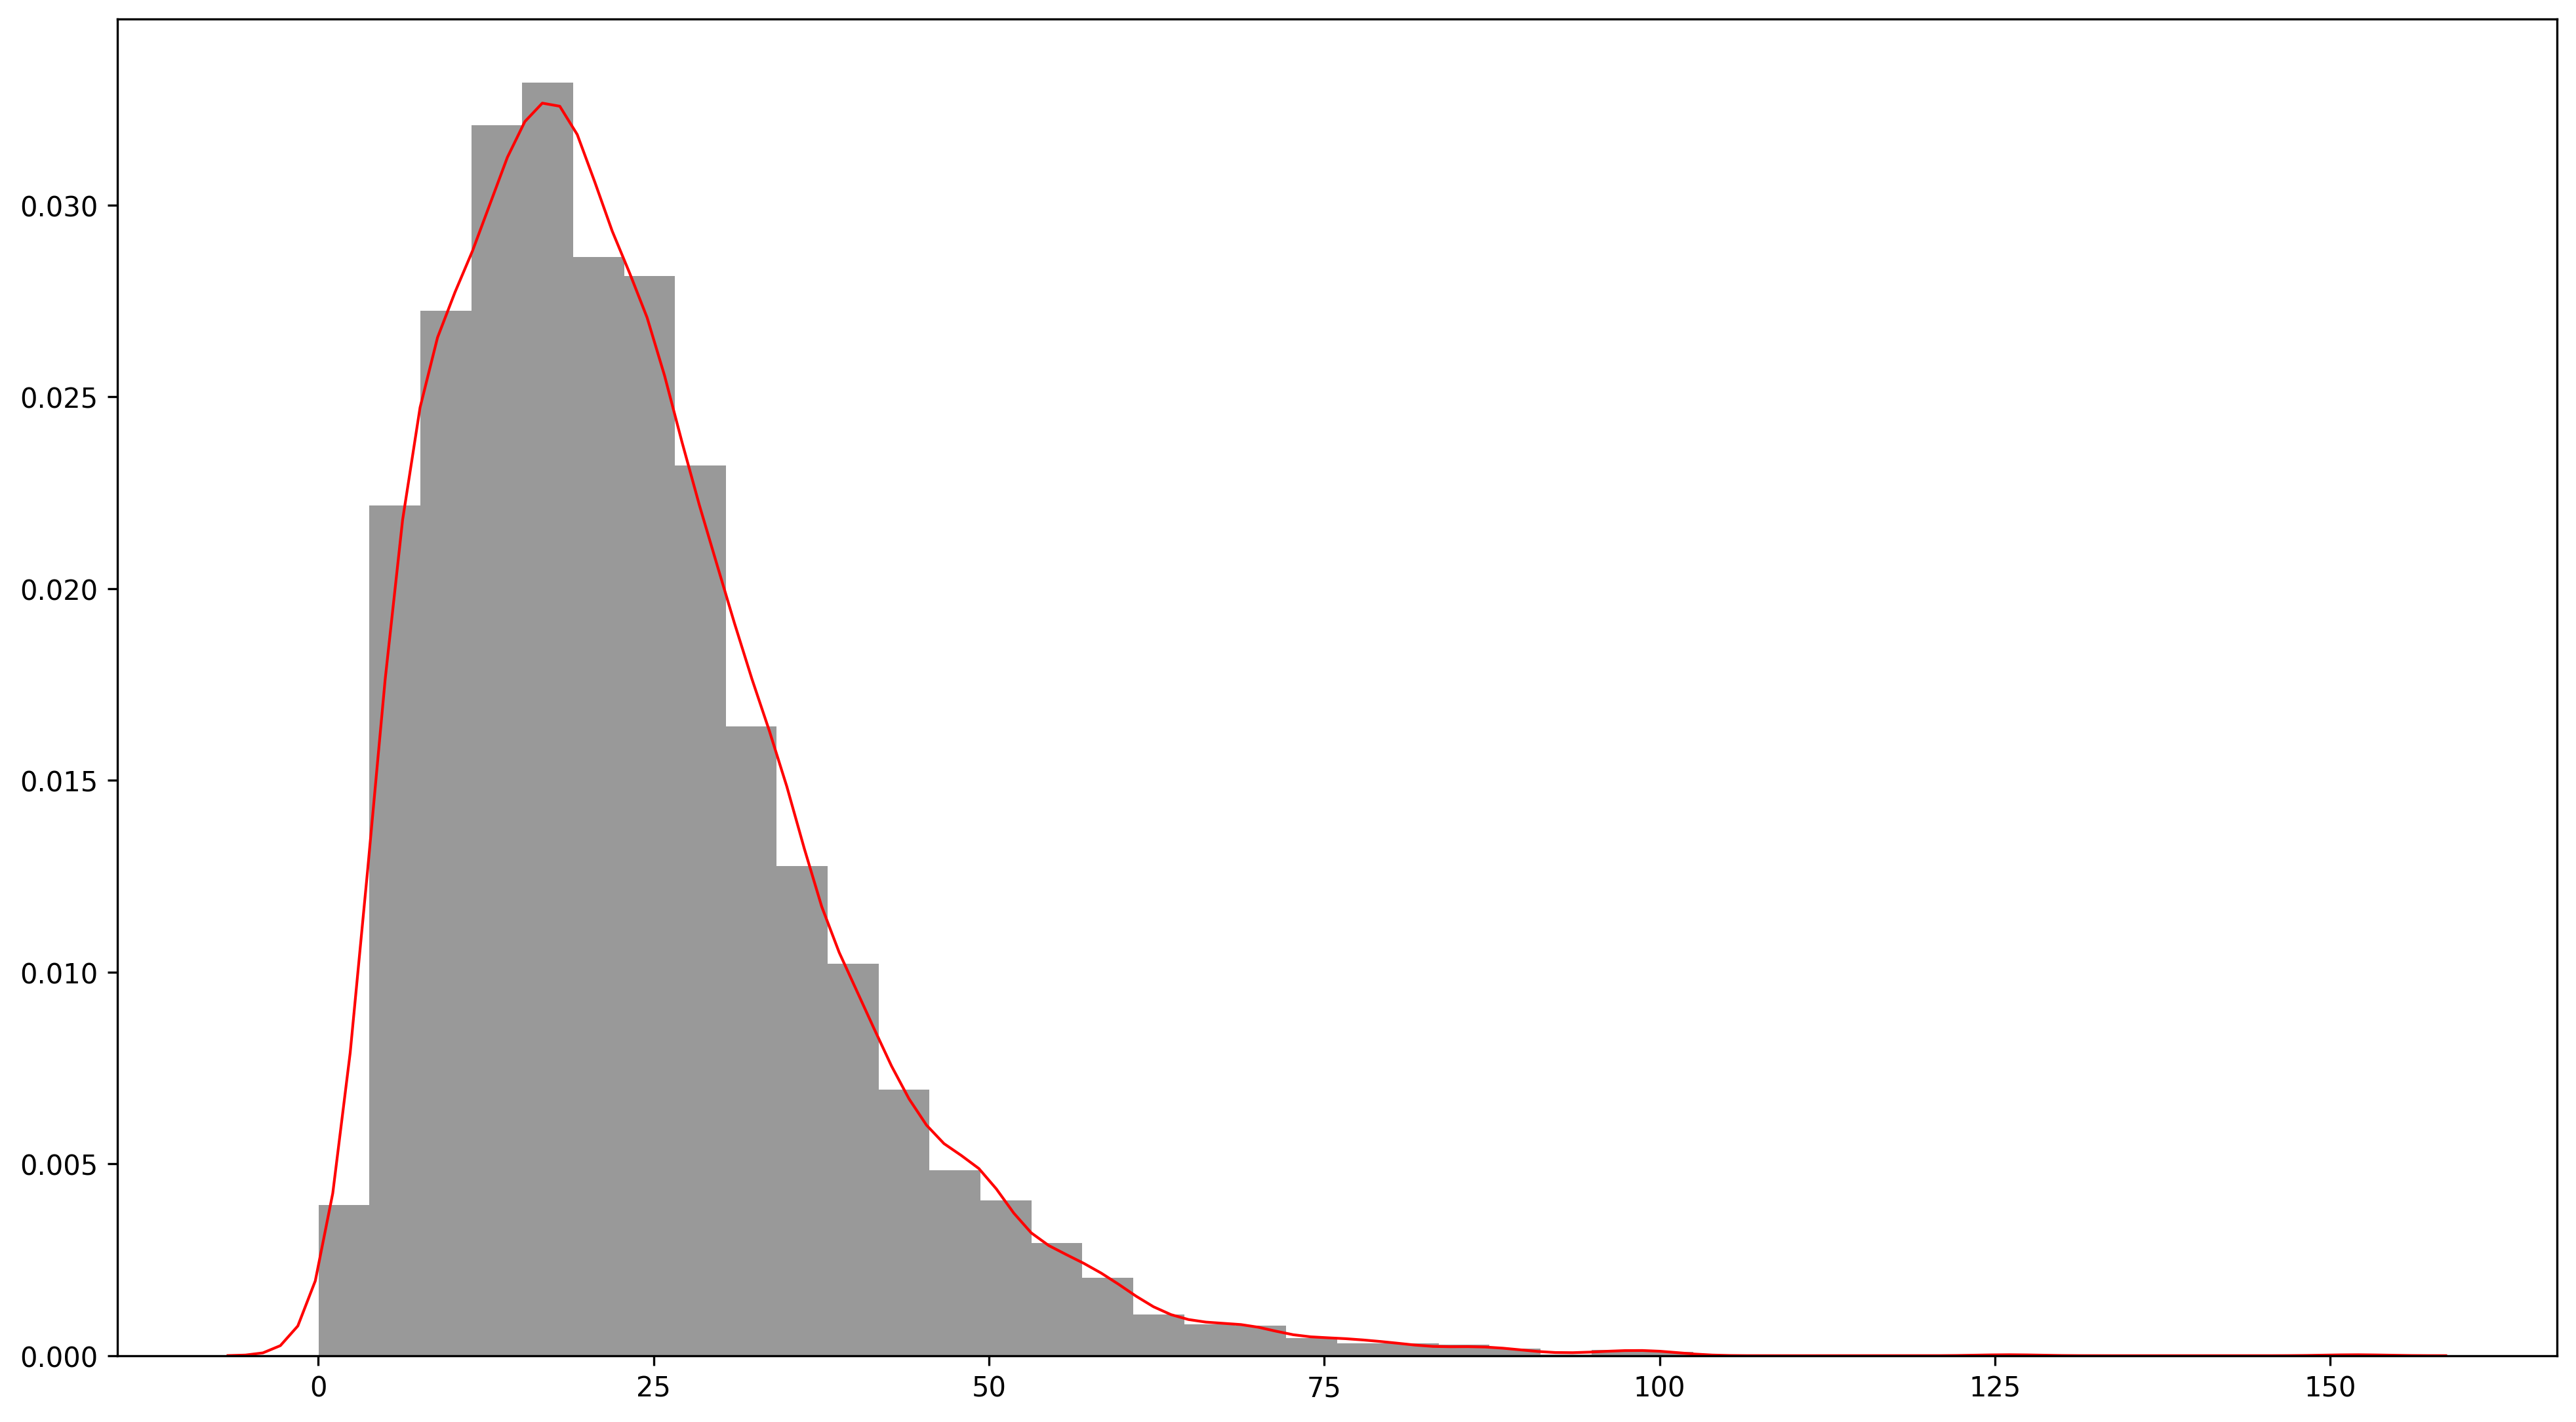
\includegraphics[width=1\linewidth]{meanprice_hist}
\end{figure}

\begin{figure}[h]
\centering
\caption{Histogram of Reviewer Ratings}
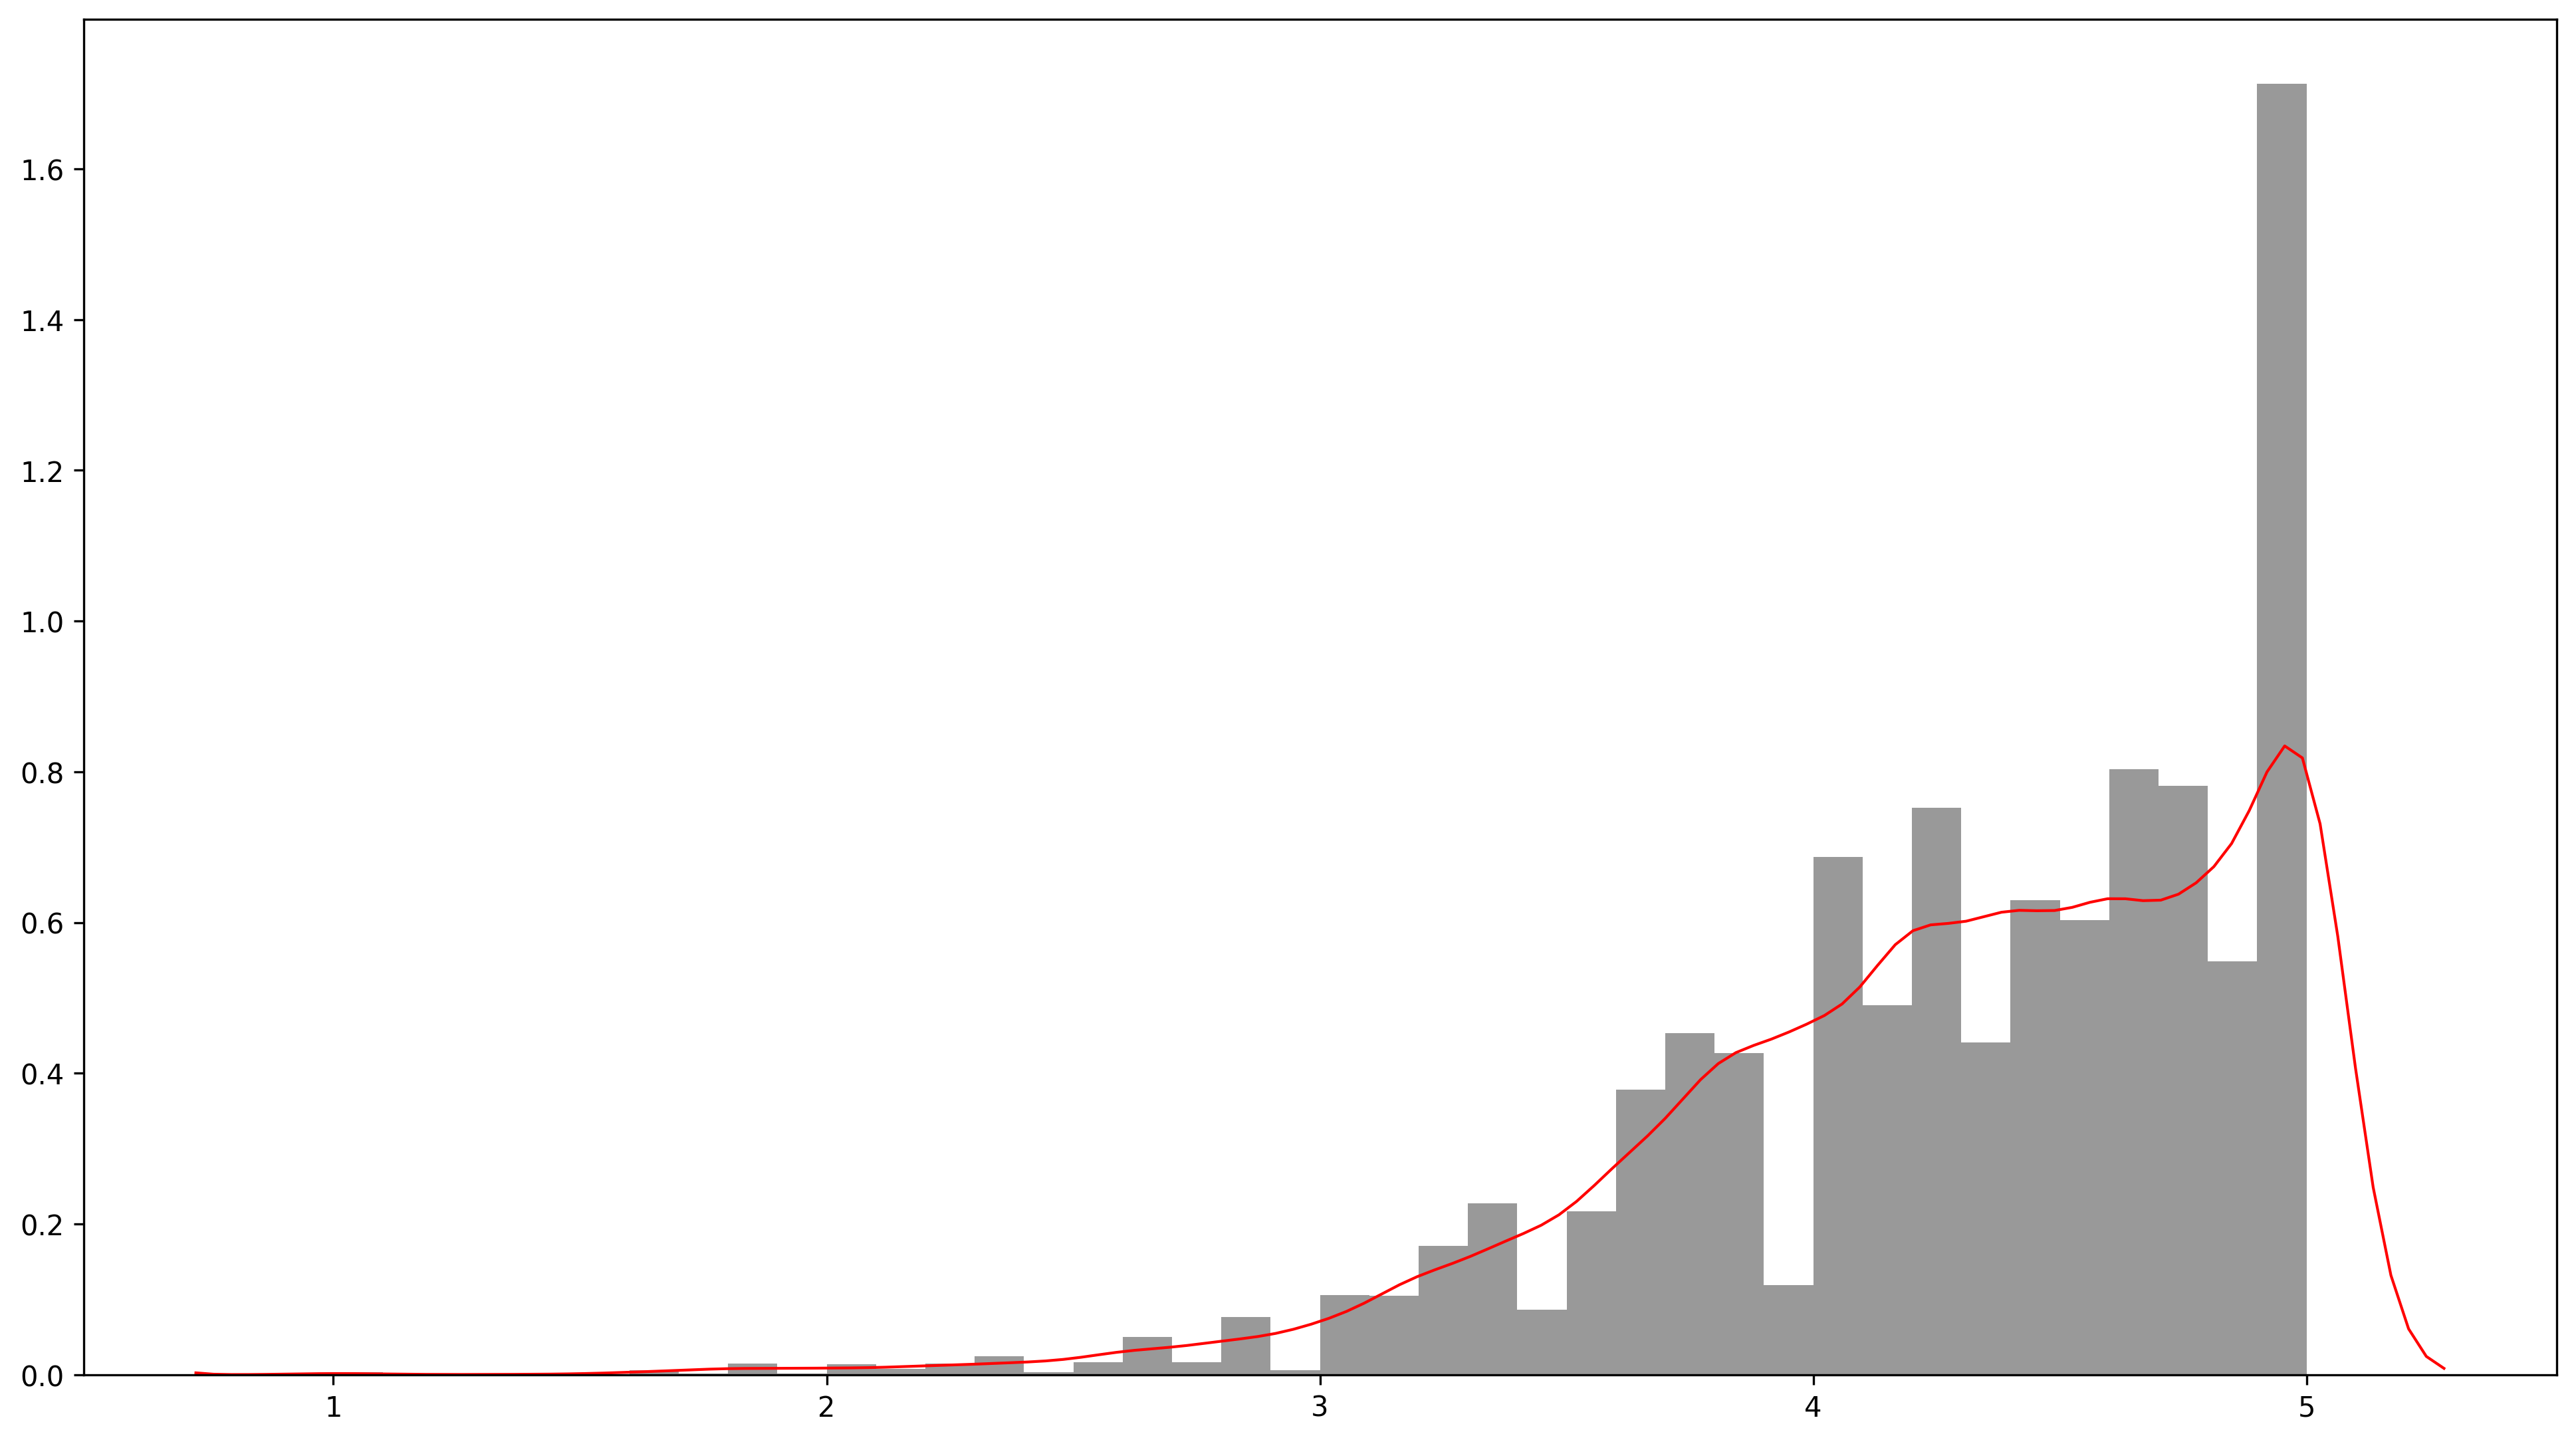
\includegraphics[width=1\linewidth]{meanstar_hist}
\end{figure}


\section{Methodology \& Model Selection}

\section{Implementation}

\section{Discussion}

\section*{Reference}

\begin{thebibliography}{0}\setlength{\itemsep}{4mm}

\bibitem{}Moe, W. (2003). Buying, Searching, or Browsing: Differentiating Between Online Shoppers Using In-store Navigational Clickstream. \textit{Journal of Consumer Psychology 13(1–2)}, pp. 29 - 39.

\bibitem{}Ricci, F., Rokach, L., \& Shapira, B. (2011). Introduction to Recommender Systems Handbook, \textit{Recommender Systems Handbook, Springer}, pp. 1 - 35.

\bibitem{}Sakar, C.O., Polat, S.O., Katircioglu, M., \& Kastro, Y. (2018). Real-time Prediction of Online Shoppers’ Purchasing Intention Using Multilayer Perceptron and LSTM Recurrent Neural Networks, \textit{Neural Computing and Applications}, pp. 1 - 16.

\bibitem{}van der Heijden, H., Verhagen, T., \& Creemers, M. (2003). Understanding Online Purchase Intentions: Contributions from Technology and Trust Perspectives, \textit{European Journal of Information System, 12}, pp. 41 - 48.

\end{thebibliography}

\end{document}
